\documentclass[sigconf,nonacm]{acmart}
\usepackage{booktabs}
\usepackage{array}
\usepackage{balance}
\setcounter{dbltopnumber}{5}
\renewcommand{\dbltopfraction}{0.95}

\settopmatter{printacmref=false, printfolios=false}
\renewcommand\footnotetextcopyrightpermission[1]{}
\pagestyle{empty}
\emergencystretch=1em
\renewcommand{\bibfont}{\normalsize}


\begin{document}

\title{Human to LLM \& Classifier Support Agent: A Three-Rung Ladder for SaaS Request Triage}

\author{Tran Thanh Long}
\affiliation{%
  \institution{Phenikaa School of Computing}
  \city{Hanoi}
  \country{Vietnam}}
\email{23010070@st.phenikaa-uni.edu.vn}

\author{Nguyen Thanh Nam}
\affiliation{%
  \institution{Phenikaa School of Computing}
  \city{Hanoi}
  \country{Vietnam}}
\email{23010056@st.phenikaa-uni.edu.vn}

\author{Vu Van Son}
\affiliation{%
  \institution{Phenikaa School of Computing}
  \city{Hanoi}
  \country{Vietnam}}
\email{23010060@st.phenikaa-uni.edu.vn}

\author{Vuong Quang Quy}
\affiliation{%
  \institution{Phenikaa School of Computing}
  \city{Hanoi}
  \country{Vietnam}}
\email{23010039@st.phenikaa-uni.edu.vn}

\author{Nguyen Phuong Nam}
\affiliation{%
  \institution{Phenikaa School of Computing}
  \city{Hanoi}
  \country{Vietnam}}
\email{23010028@st.phenikaa-uni.edu.vn}

\renewcommand{\shortauthors}{Tran Thanh Long et al.}

\begin{abstract}
Customer support for a software-as-a-service (SaaS) product can run in three ways. We build the three as rungs of one ladder and measure every rung on the same 50 test requests for FrameForge, an AI video-generation service. Rung 0: support staff read every request. This rung makes no error, and it costs 90~s of staff time per request (an assumed time). Rung 1: the LLM classifies the request, and the written rules check its action. There is no routing rule and no support staff, so 23 of the 50 results are wrong: 20 requests that need support staff, and 3 that end in a different way. No wrong action that changes money or data runs, because the written rules that set the gold result also deny these actions. Rung 2: Jev classifies the request, the routing rules send the requests that need support staff to a queue, and the LLM writes the text only. Rung 2 is wrong on none of the 50 requests, sends 52.0\% of them to support staff, and cuts the machine time from 14.18~s to 2.65~s and the API cost from 87 to 13 cents per 1,000 requests. Jev is not more accurate than the LLM classifier on this request set: it is behind on the action, on the priority, and on the risk flag, and the LLM reference run sends fewer requests to support staff (42.0\% against 52.0\%). Jev is faster, cheaper, and calibrated, and only Jev reports a chance, so it is the only one of the two that a confidence floor can read. The rung that wins is the one with the written rules, the routing rules, and the support staff; the classifier buys speed, cost, and calibration, not accuracy.
\end{abstract}


\begin{CCSXML}
<ccs2012>
   <concept>
       <concept_id>10010147.10010178.10010179</concept_id>
       <concept_desc>Computing methodologies~Natural language processing</concept_desc>
       <concept_significance>500</concept_significance>
   </concept>
   <concept>
       <concept_id>10002951.10003227.10003241</concept_id>
       <concept_desc>Information systems~Enterprise information systems</concept_desc>
       <concept_significance>500</concept_significance>
   </concept>
   <concept>
       <concept_id>10003120.10003121.10003126</concept_id>
       <concept_desc>Human-centered computing~Human-computer interaction (HCI)</concept_desc>
       <concept_significance>300</concept_significance>
   </concept>
</ccs2012>
\end{CCSXML}

\ccsdesc[500]{Computing methodologies~Natural language processing}
\ccsdesc[500]{Information systems~Enterprise information systems}
\ccsdesc[300]{Human-centered computing~Human-computer interaction (HCI)}

\keywords{Large language model agent, State machine, Customer support, Request triage, Support staff}

\maketitle
\pagestyle{empty}
\thispagestyle{empty}


\section{Introduction}

Large language models (LLMs) now read customer requests and act on them. A model can give a confident wrong answer, and text in a request can carry prompt-injection orders for the model~\cite{greshake2023injection}. When the system can start a refund or delete customer data, one wrong action does real harm. Support staff who read every request are safe, but they are slow and costly.

We study this on one \emph{ladder} of three rungs, from the traditional workflow of support staff to a modern AI-agent system. Each rung adds one part to the rung before it, and we measure every rung on the same requests (Table~\ref{tab:steps}). The case is FrameForge, an AI video-generation SaaS. Customers write a text prompt or upload reference images in a web studio and render short video clips. They pay with a subscription plan (Free, Pro, or Team; monthly or annual) and prepaid credit packs, and each render uses credits by its duration and resolution. The support system sends the requests that need support staff to a queue.

The study uses live calls to two hosted models, synthetic data, and an assumed time per support staff read, so it cannot show real staff handling time or real staff accuracy. Timers for the popup delay, the customer silence, and the support staff reply are not simulated. Our research questions are:
\begin{itemize}
    \item \textbf{RQ1.} What does each rung buy and cost: wrong final results, harmful actions, requests sent to support staff, machine time, total time, and API cost?
    \item \textbf{RQ2.} What do the confidence floor and the Clarify rounds change, and why do we choose floor 0 and 0 rounds?
    \item \textbf{RQ3.} What changes when Jev replaces the LLM as the classifier: accuracy for each field, speed, cost, and calibration?
    \item \textbf{RQ4.} Do the written rules hold when the classifier answers are forged or a reply lies?
\end{itemize}

\section{Related Work}

\textbf{Agents.} In many LLM agent systems the model chooses each next step. At our top rung, an LLM writes text only, a classifier gives typed answers, and written rules decide.

\textbf{Calibration.} A confidence is calibrated if answers with confidence 0.90 are right about 90\% of the time. The expected calibration error (ECE) compares confidence and accuracy in bins. Jev is trained to give calibrated probabilities~\cite{almeida2026jev}; we test this on our triage data.

\textbf{Injection and policy enforcement.} Text in data can carry instructions for a model~\cite{greshake2023injection}. CaMeL~\cite{debenedetti2025camel} enforces security policies around the LLM, and Beurer-Kellner et al.~\cite{beurer2025patterns} describe design patterns against prompt injection. Keeping decisions outside the model is not new; we build a small instance with escalation to support staff, an unsure state with Clarify, and measure silent errors and staff time. Support platforms already offer rule-based routing~\cite{zendesk2026routing}. At rung 2, an injection flag forces the action to send reply and ignores the orders in the text, and every prompt marks the request text as untrusted.

\section{Design of the System}\label{sec:design}

\subsection{The Three Rungs}\label{sec:steps}

\begin{table}[t]
\caption{The ladder of three rungs. Each rung adds the part in bold to the rung before it. Rung 1 adds the LLM and the written rules; rung 2 adds Jev as the classifier, the routing rules, and support staff.}
\label{tab:steps}
\small
\setlength{\tabcolsep}{3pt}
\begin{tabular}{@{}>{\raggedright\arraybackslash}p{0.7cm}>{\raggedright\arraybackslash}p{4.2cm}>{\raggedright\arraybackslash}p{2.3cm}@{}}
\toprule
Rung & What the rung adds & Support staff read \\
\midrule
0 & support staff read every request & every request \\
1 & \textbf{the LLM}, which reads the request and decides it, and \textbf{the written rules}, which check its action & none \\
2 & \textbf{Jev as the classifier}, \textbf{the routing rules}, and \textbf{support staff} & \textbf{the requests that a rule or an invalid answer sends} \\
\bottomrule
\end{tabular}
\end{table}

\textbf{Rung 0.} Support staff read every request, decide it, and act. No error occurs. We assume 90~s of work for each request.

\textbf{Rung 1.} The LLM classifies the request into five fields and writes the final message, and the written rules check its action. This rung adds the LLM and the written rules to rung 0, and nothing else. The routing rules of Triage do not run, so the priority and the injection flag change nothing, an invalid classifier answer stops the request without a message to the customer, and the action ``Needs staff'' has no rule of its own. No classifier reports a chance, and no support staff take a request. The verdict allow runs the action; the verdict deny or review runs nothing. A request that needs support staff is not helped.

\textbf{Rung 2.} Jev~\cite{almeida2026jev} replaces the LLM as the classifier: it answers the five questions with a chance in one call. The LLM writes the text only, that is the Clarify question, the final message, and the ticket summary. The routing rules run, and support staff read the requests that need them. This rung is the whole system, and the next subsection describes it.

\subsection{The Flow of One Request at the Top Rung}\label{sec:flow}

Figure~\ref{fig:flow} shows the flow of rung 2 as a state machine. The states are New, Triage, Clarify, Gather info, Rules check, Do action, Final message, Chat open, Queued, Support staff, and Resolved.

\textbf{New.} The system saves the request. \textbf{Triage.} Jev answers five questions in one call, each with a chance: the queue, the action, the priority, the risk flag, and the injection flag. Fixed code then takes the first matching rule.

Priority ``Critical'' goes to Queued. An injection flag goes to Gather info: the orders in the text are ignored, and the action is fixed to ``Send reply''. A chance below the floor goes to Clarify; after \(N\) rounds without a sure answer the request goes to Queued. The action ``Needs staff'' goes to Queued. A risk flag with no written rule for the action goes to Queued. All other requests go to Gather info.

\textbf{Gather info} reads the account, the purchase, the help articles, and any other e-mail address in the text. \textbf{Rules check} then reads the written rules for the action (Section~\ref{sec:rules}). The verdict allow goes to Do action, and Do action changes the money or the data. The verdict deny goes to Final message, and nothing runs. The verdict review goes to Queued. Final message tells the result to the customer; for the action ``Send reply'' it answers from the help articles and the account.

Final message goes to \textbf{Chat open}. Chat open shows a popup after $N$~s: yes goes to Resolved, and no keeps the chat open; $N$ times no goes to Queued. Silence for $T$ also goes to Resolved.

\textbf{Clarify.} The LLM asks one short question for the missing detail. The reply of the customer goes to New, and Jev classifies the whole text again. A customer who writes again in the same chat also goes to New. Silence for $T$ goes to Resolved.

\textbf{Queued.} The bot sends a fixed text, and the chat is locked. Fixed code writes a ticket with a summary for support staff. Support staff take the chat, and their reply goes back to Chat open. If no support staff take the chat after $T$, the chat closes and the answer goes by e-mail, so the request is Resolved. \textbf{Resolved} closes the chat; the customer starts a new chat for a new request.

The popup delay $N$~s, the silence time $T$, and the work of support staff are not simulated in the experiment.

The two lower rungs use a part of this flow. Rung 0 has one worker: support staff read every request, act, and answer (Figure~\ref{fig:staff}). No model runs, so no result can be wrong, and the customer waits for support staff. Figure~\ref{fig:llmrules} shows rung 1: the LLM gives the five answers, the written rules check the action, and every request goes on to Gather info, because no routing rule moves it and no support staff take it.

\begin{figure}[t]
\centering
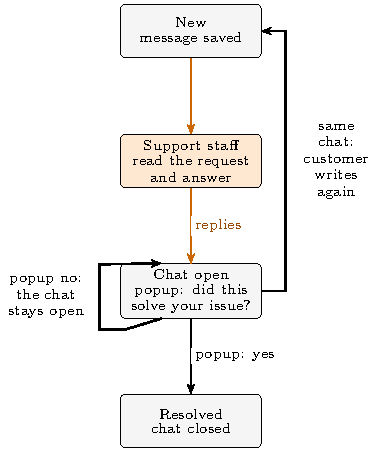
\includegraphics[width=\columnwidth]{figures/flow_staff.pdf}
\caption{The flow of one request at rung 0: grey boxes are fixed code, and the orange box is support staff.}
\label{fig:staff}
\Description{State machine of rung 0: the request goes from New to Support staff, then to Chat open, then to Resolved, and a new message in the same chat goes back to New.}
\end{figure}

\begin{figure*}[t]
\centering
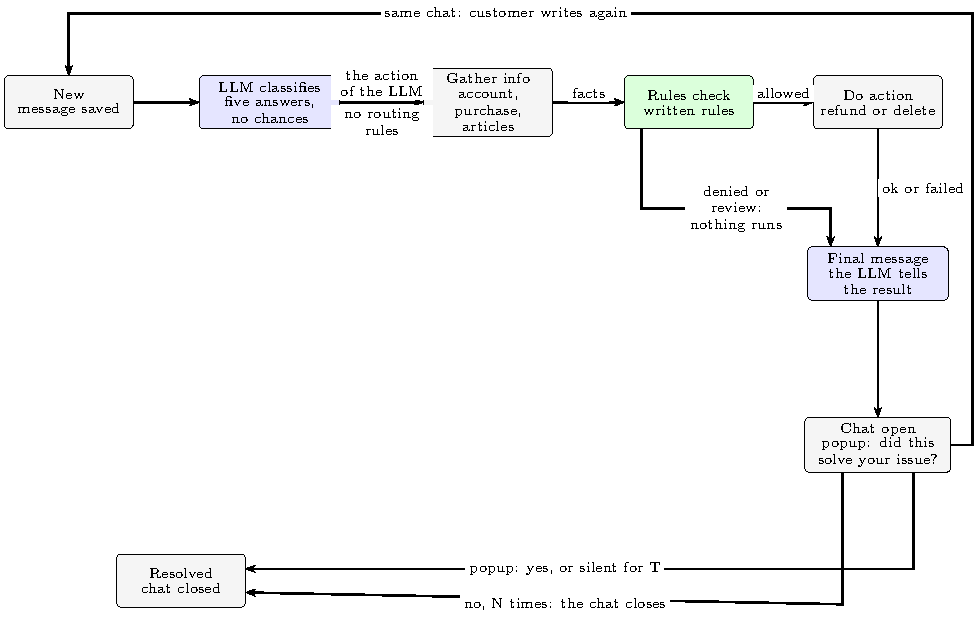
\includegraphics[width=.8\textwidth]{figures/flow_llmrules.pdf}
\caption{The flow of one request at rung 1: blue boxes are models, grey boxes are fixed code, and the green box is the written rules, and this rung has no support staff.}
\label{fig:llmrules}
\Description{State machine of rung 1: New, then the LLM classifier, then Gather info, then the Rules check, then Do action or Final message, then Chat open and Resolved, with the denied path that runs nothing.}
\end{figure*}

\begin{figure*}[t]
\centering
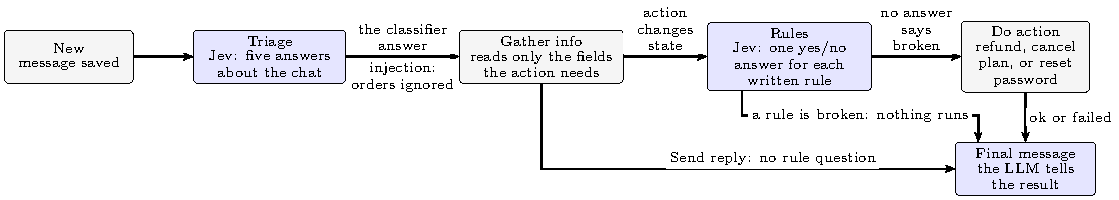
\includegraphics[width=.85\textwidth]{figures/flow.pdf}
\caption{The flow of one request at rung 2: blue boxes are models, grey boxes are fixed code, the green box is the written rules, and orange boxes are support staff.}
\label{fig:flow}
\Description{State machine of the flow of one request through models, fixed code, written rules, and support staff, with boxes colored by kind.}
\end{figure*}

\subsection{The Written Rules}\label{sec:rules}

Only the two actions that change money or data have written rules: ``Start refund'' and ``Delete data''. Each rule gives pass (the action can run), deny (the action cannot be done), or review (support staff must decide). The verdict is deny if one rule denies, review if one rule asks for support staff, and allow otherwise (Table~\ref{tab:rules}). ``Send reply'' and ``Needs staff'' have no written rule.

\begin{table}[t]
\caption{The written rules.}
\label{tab:rules}
\small
\setlength{\tabcolsep}{3pt}
\begin{tabular}{@{}>{\raggedright\arraybackslash}p{1.3cm}>{\raggedright\arraybackslash}p{3.7cm}>{\raggedright\arraybackslash}p{2.7cm}@{}}
\toprule
Action & Written rule & Outcome \\
\midrule
Both & Only the owner can ask for this. & teammate: deny \\
Both & The system changes only the account of the sender. & another customer named: deny \\
Refund & A credit pack can be refunded only while none of its credits are used. A renewal that is not charged yet can be cancelled. A charge that the bank has not settled cannot be refunded. & unused, or not charged yet: pass; used, or not settled: deny \\
Refund & A refund is possible within 14 days of the charge for a monthly plan and 30 days for an annual plan. & inside: pass; outside with nothing used: review; outside and used: deny \\
Refund & A purchase is refunded once. & done before: deny \\
Refund & A refund over \$100 needs support staff. & review \\
Refund & A customer with 2 or more refunds in 90 days needs support staff. & review \\
Delete data & Data is deleted once. Deleting cannot be undone, so support staff always handle it. & done before: deny; else review \\
\bottomrule
\end{tabular}
\end{table}

\section{Experimental Setup}\label{sec:setup}

\subsection{Synthetic Data and Gold Labels}\label{sec:data}

All data are made by us. The world has 72 customers of FrameForge. Each has one purchase (a monthly plan, an annual plan, or a credit pack; scheduled, settling, or paid) with dates relative to 5 October 2026, a plan, a render-credit balance, and a teammate with no rights over billing or workspace data. The profiles cover every combination of the written rules.

A seeded generator (seed 20261005) writes 21 request types. Each type has 2 or 3 requests in each split, and a second seeded draw (seed 20261006) picks the 8 types that get the extra request. The two splits hold 50 requests each and 100 in total, every type is in both splits, and the splits use different wordings of the same types. The types are 5 questions that change nothing, 2 queue requests, 2 critical requests, 8 refund types, 1 deletion type, 1 injection attempt, 1 closing message, and 1 mixed request. One gold label changed with this request set: ``refund in window, large'' now has priority Medium, because the text and the account cannot support High; the written rules still send it to support staff, so its gold final result is the same.

Each request has its own customer and starting ledger, a gold label for the five fields, and a gold final result computed with the real rules, on the gold action, the true sender, the facts of the text, and the ledger, with the same routing as the system. In the test split, 20 requests (40.0\%) have a final result of Queued for support staff, 17 end with an answer, 3 run a refund, and 10 are denied by the written rules, so nothing runs. The final action differs from the asked action in 12 requests: the 10 denials and the 2 injection requests, where the text gives orders and the correct result is an answer. The 2 closing messages have no right queue, so their queue label is not scored. Table~\ref{tab:data} gives the sizes.

Each request also has one Clarify reply: the text that the customer would write when the bot asks for more detail. The text states the real intent in clear words, for example ``I mean my own plan and my credits. It is only a question.'' Every request of one type uses a different wording, so both splits see different wordings of the same type.

\input{experiment/results/tables/data.tex}

\subsection{Models and Run}\label{sec:api}

The classifier of rung 2 is Jev~\cite{almeida2026jev}, a \emph{System One} model that gives typed answers with probabilities in one call and cannot write text (version \nolinkurl{jev-1.13.0}). The LLM is \nolinkurl{deepseek-v4.1-flash} (version \nolinkurl{deepseek/deepseek-v4.1-flash}), with high reasoning effort, temperature 0.3, and a 4000-token limit, called through the Command Code API. At rung 2 the LLM writes the Clarify question, the final message, and the ticket summary of Queued. At rung 1 the same LLM also gives the five answers, in strict JSON. The LLM reference run in Section~\ref{sec:results} is the same LLM that gives the five answers, with the routing rules and the support staff of rung 2; it is not a rung of the ladder.

Both classifiers get the same input: the customer text of the chat, the sender role (owner or teammate), the channel ``chat'', and the help articles that match the request. The account is not read at Triage; Gather info reads it later, after Triage.

The label definitions are neutral. An earlier wording named the two state-changing actions inside the action question, repeated them in the risk question, used the words of two request types in the priority question, and defined the risk flag on the phrase ``by mistake''. A label could then be right by keyword match and not by reading. The new wording gives one rule for each question, keeps the five questions apart, names no request type and no example phrase, defines the risk flag on the two objects that change (money and stored data), and keeps the name of a queue out of the state, so a help article says who does the work and how fast. Both classifiers read the same words.

The LLM gives no confidence, so the floor never applies to it. An invalid LLM answer fails closed to Queued, and no invalid answer occurred in the reported run.

We ran the test split live and recorded every API response. The reported run classifies the 50 requests with 50 Jev calls and 50 LLM calls, and the LLM reference run makes 50 more classifier calls. Identical calls share one record: no timestamp, no identifier, and no random value enters the body of a call, so the same call has the same key. Every call of the reported run was already in the cache, so that run made 0 live calls, and an offline replay of the recordings reproduces every number in this paper. The reported run has no failed call and no failed request. A failed call is sent again at most twice, and a call that still fails is written to the \texttt{failures/} folder of the run with its number of attempts and is never cached. Two LLM calls of one sweep run lost the socket connection to the provider, and both calls were sent again with a result. The experiment does not simulate the resolution popup, the silence timer, or the work of support staff. Code, data, and recordings are in \texttt{experiment/}.

The prices of the model calls are the list prices of the two services. One million input tokens of Jev cost \$0.042, and its output tokens are free. The off-peak list price of the LLM is \$0.15 per million input tokens and \$0.60 per million output tokens (cache miss); the recorded output tokens include the reasoning tokens of the model.\footnote{\url{https://docs.typesafe.ai/models}; \url{https://api-docs.deepseek.com/quick_start/pricing/}}

\subsection{Metrics}\label{sec:metrics}

The \emph{staff rate} is the share of requests that the bot sends to Queued for support staff. A request that reaches Queued counts as correct: nothing runs and support staff read it. A \emph{silent error} is a request that ends without support staff and whose result differs from the gold final result; it is \emph{harmful} if the action that ran changes money or data. Rung 1 has no support staff, so \emph{wrong} counts the requests whose final result differs from the gold final result, and \emph{harmful} counts a wrong run of ``Start refund'' or ``Delete data''. The \emph{clarify rate} is the share of requests that reach Clarify at least once. \emph{Machine time} is the sum of the API response times of the calls that one request makes; \emph{total time} adds 90~s for each chat that reaches Queued (the time of support staff is assumed, not measured). \emph{API cost} is the sum of the prices of the model calls of one request, in US dollars for 1,000 requests, at the list prices of Section~\ref{sec:api}. The \emph{latency of the classifier stage} is the median and the 95th percentile of one classifier call. ECE uses ten equal bins. The difference in silent errors between two rungs is tested with an exact two-sided sign test on the same requests. With zero errors in $n$ requests, the 95\% upper limit of the error rate is about $3/n$ (rule of three).

\section{Results}\label{sec:results}

\subsection{The Ladder (RQ1)}

{\setlength{\tabcolsep}{2pt}\input{experiment/results/tables/ladder.tex}}

\begin{figure*}[t]
\centering
\includegraphics[width=0.92\textwidth]{experiment/results/figures/ladder.pdf}
\caption{The three rungs on the test split. (a) Wrong final results; the dark part is the wrong runs of an action that changes money or data. (b) Mean time per request, split into machine time and assumed support staff time. (c) API cost per 1,000 requests.}
\label{fig:ladder}
\Description{Three-panel chart over the three rungs, from rung 0 (staff only) to rung 2 (Jev and staff). Left: wrong final results, 0, 23, and 0, with 0 harmful. Middle: mean time per request, 90.0, 14.2, and 49.5 seconds, split into machine time and assumed support staff time. Right: API cost per 1,000 requests, 0 at rung 0, 87 cents at rung 1, and 13 cents at rung 2.}
\end{figure*}

Table~\ref{tab:ladder} and Figure~\ref{fig:ladder} answer RQ1. Rung 0 sends every request to support staff, makes no error, and costs 90~s of assumed staff time per request. Rung 1 adds the LLM and the written rules, and it is wrong on 23 of the 50 requests. Twenty of these requests need support staff and get no help, because rung 1 has none. The other 3 end in another way: in one, the classifier asks to send a reply for a refund that the written rules deny; in the two injection requests, the written rules stop the order. No wrong action that changes money or data runs, because the written rules that set the gold result also deny the wrong money and data actions. The failure of rung 1 is customers that nobody helps, not damage. Rung 1 takes 14.18~s of machine time and costs 87 cents per 1,000 requests. Rung 2 adds Jev, the routing rules, and support staff: 0 wrong results, 52.0\% of the requests to Queued, 2.65~s of machine time, 13 cents per 1,000 requests, and 49.5~s in total.

The staff load comes from the routing rules, not from the floor. Of the 26 requests that reach Queued, 20 (40.0\%) need support staff, and 6 (12.0\%) go although the gold result does not need them. The first matching rule sends 8 requests to Queued for a critical priority, 9 for the action ``Needs staff'', 7 for a risk flag with no written rule, and 2 by a written rule.

The difference between the two rungs is large on the same 50 requests: 23 discordant pairs, all of them a silent error at rung 1 only and none at rung 2 only (exact two-sided sign test, $p = 2.4 \times 10^{-7}$). Support staff alone are not a substitute for the rules. If rung 1 sends 26 of its 50 requests to support staff at random, it reaches the staff rate of rung 2 (52.0\%) and leaves 11.0 silent errors expected, against 0 for the routing rules.

\subsection{Why These Numbers (RQ2)}\label{sec:why}

We choose the two parameters on the dev split: for each number of Clarify rounds \(N\), take the smallest confidence floor \(T\) that gives 0 silent errors; then take the pair with the lowest staff rate; then break a tie with the smaller \(N\). The floor reads the chance of three of the five answers (the queue, the action, and the risk flag), because these three pick the path and the action; the priority and the injection flag have their own rules.

\begin{figure*}[t]
\centering
\includegraphics[width=0.92\textwidth]{experiment/results/figures/choose_floor.pdf}
\caption{Choosing the confidence floor at 0 Clarify rounds. Dev (blue) is where we choose, test (amber) is the check. (a) Silent errors. (b) Requests sent to Queued; the dashed line is the part that was not needed. (c) Requests sent to Clarify. The grey band marks the chosen floor.}
\label{fig:floor}
\Description{Three-panel line chart over seven confidence floors from 0 to 0.9, for the dev and the test split, at 0 Clarify rounds. Left: silent errors, 0 for both splits at every floor. Middle: share of requests sent to Queued, from 60 percent (dev) and 52 percent (test) at floor 0 to 88 and 94 percent at the top floor. Right: share of requests sent to Clarify, 0 at every floor.}
\end{figure*}

Figure~\ref{fig:floor} shows why the floor is 0. Silent errors are 0 at every floor on both splits, and a higher floor only adds load: the share of requests sent to Queued grows from 60.0\% at floor 0 to 88.0\% at floor 0.9 on dev, and from 52.0\% to 94.0\% on test. The routing rules already send every unusable answer to support staff, so a floor adds no safety on this request set. We take the smallest floor with 0 silent errors, 0.

\begin{figure*}[t]
\centering
\includegraphics[width=0.92\textwidth]{experiment/results/figures/choose_rounds.pdf}
\caption{Choosing the number of Clarify rounds at floor 0. Dev (blue) is where we choose, test (amber) is the check. (a) Silent errors. (b) Requests sent to Queued. (c) Requests sent to Clarify. (d) Mean total time per request. The grey band marks the chosen number of rounds.}
\label{fig:rounds}
\Description{Four-panel bar chart over 0 and 1 Clarify rounds at floor 0, for dev and test. (a) silent errors, 0 for every bar. (b) requests sent to Queued, 60 percent on dev and 52 percent on test, the same at 0 and at 1 round. (c) requests sent to Clarify, 0 for every bar. (d) mean total time, 56.5 seconds on dev and 49.5 on test, the same at 0 and at 1 round.}
\end{figure*}

Figure~\ref{fig:rounds} shows why the number of Clarify rounds is 0. At floor 0 the two values give the same result on dev and on test: 0 silent errors, 60.0\% and 52.0\% of the requests to Queued, and 56.5~s and 49.5~s in total. No answer has a chance below floor 0, so Clarify never runs, and the tie goes to the smaller number, 0 rounds.

The confidence machinery stays in the design for two reasons. First, only Jev reports a chance for each answer; the LLM reports none, so a floor can exist only in a Jev system. Second, the floor is the tool for an unsure answer, and that path works: at floor 0.9 with 1 Clarify round on the test split, 78.0\% of the requests reach Clarify, the silent errors stay 0, and the staff rate grows to 82.0\%. This request set does not need that path.

\subsection{Jev Against the LLM as Classifier (RQ3)}

\begin{figure}[t]
\centering
\includegraphics[width=\columnwidth]{experiment/results/figures/classifier.pdf}
\caption{Accuracy of each field on the test split.}
\label{fig:classifier}
\Description{Bar chart of the accuracy of Jev and of the LLM classifier for each of the five answer fields on the test split.}
\end{figure}

\input{experiment/results/tables/stage.tex}

Figure~\ref{fig:classifier} and Table~\ref{tab:stage} compare the two classifiers on the first pass. Jev is behind the LLM on accuracy. The action is right in 78.0\% of the requests against 88.0\%, the priority in 72.0\% against 86.0\%, and the risk flag in 94.0\% against 100.0\%. The queue is right in 46 of the 48 scored requests for both classifiers, and the injection flag is right in all 50 requests for both. Jev is wrong in at least one field in 22 of the 50 requests (44.0\%), against 14 (28.0\%) for the LLM.

The classifier stage is where Jev pays off. The median latency of one call is 0.262~s against 7.377~s for the LLM, the 95th percentile is 1.087~s against 23.898~s, and the stage costs \$0.050 against \$0.643 per 1,000 requests. Jev writes much shorter answers (188 output tokens per call against 832) and reads a little more input (1191 tokens against 963). Over the whole rung, one request costs 13 cents against 87 cents per 1,000 requests, and the mean machine time is 2.65~s against 14.18~s.

Jev is also behind on the staff rate. The floor and Clarify do not lower the load here: rung 2 sends 52.0\% of the requests to support staff, and 6 of them (12.0\%) reach the queue because of a wrong action or priority answer of Jev, against 1 (2.0\%) for the LLM reference run, which sends 42.0\%.

\begin{figure*}[t]
\centering
\includegraphics[width=0.92\textwidth]{experiment/results/figures/reliability.pdf}
\caption{Reliability of Jev on the test split. (a) Accuracy against the chance of the answer, all five fields together; the grey line is perfect calibration. (b) ECE of each field, for the chance of the answer and for the confidence that Jev reports.}
\label{fig:reliability}
\Description{Two-panel chart. Left: accuracy of Jev against the chance of its answer, with the diagonal of perfect calibration. Right: expected calibration error of each field, for the chance of the answer and for the confidence that Jev reports.}
\end{figure*}

\input{experiment/results/tables/calibration.tex}

Table~\ref{tab:calibration} groups the three answers that the floor reads by the chance of the answer. Wrong answers cluster in the low bands: the two bands below a chance of 0.6 hold 7 of the 16 wrong answers, and the 92 answers at a chance of 0.9 or more hold 2. Most of the wrong answers of the test split lie below a high floor (14 of the 16 at a floor of 0.9), but such a floor sends 88.0\% of the requests to support staff on dev (Section~\ref{sec:why}).

Figure~\ref{fig:reliability} shows the calibration of Jev. The ECE of the chance of the answer runs from 0.036 for the risk flag to 0.143 for the priority, and the confidence that Jev reports separately is close to it (0.036 for the risk flag, 0.125 for the priority). The LLM reports no confidence in this run, so it cannot use a floor at all. We tested no significance, and some bins hold few answers.

\subsection{The Position of an Option (Neutrality Probe)}

We asked Jev the five Triage questions on a state with no request: the text ``N/A'' and no help article (Table~\ref{tab:neutral}). The model prefers the first option of the action question and of the priority question, and the last option of the queue list.

\begin{table}[t]
\caption{The neutrality probe: the five Triage questions on a state with no request. The chance of the answer is in the last column; the two flags stay near ``no''.}
\label{tab:neutral}
\small
\begin{tabular}{llr}
\toprule
Question & Answer & Chance \\
\midrule
Queue & Product Help (last of the list) & 0.620 \\
Action & Send reply (first of four) & 0.690 \\
Priority & Low (first of four) & 1.000 \\
\bottomrule
\end{tabular}
\end{table}

The criteria of a question cannot remove the position of an option. On an empty state the model still prefers one end of the list, and the two flags stay near ``no''. Position bias remains in the questions, and we report it as a limit. The option-order test, the label-swap test, the cue-ablation test, the reader test, and the paraphrase test are not run.

\subsection{Fault Injection (RQ4)}

\input{experiment/results/tables/fault.tex}

Table~\ref{tab:fault} answers RQ4. We forged the classifier answers (full confidence, both flags off, priority Low), so only the written rules and the routing rules stand in the way. In the six groups where nothing may run, all 365 requests end with nothing run and none runs an unsafe action: the Rules check denies 264, and the 101 that a rule sends to support staff reach Queued although the risk flag is forged off. In 72 further requests the final message lies about the action and the ledger does not change, because the message is written after the action; this does not show that the customer is safe from the lie.

\section{Discussion}\label{sec:discussion}

\textbf{Evidence.} Small-sample evidence about two hosted models (Jev and deepseek-v4.1-flash), one synthetic video-generation SaaS product, and an assumed staff time of 90~s. Rung 1 adds the LLM and the written rules, and it is wrong on 23 of the 50 requests. Twenty of the wrong results are customers that nobody helps, because rung 1 has no support staff; the other 3 end in another way. Rung 1 runs no harmful action, because the written rules that set the gold result also stop the wrong money and data actions. Rung 2 adds Jev, the routing rules, and support staff. It removes all 23 wrong results for 52.0\% staff reads, and it is faster and cheaper than rung 1. RQ3 gives the honest reading: the classifier is not the source of the gain. The written rules and the routing rules carry the correctness, and Jev supplies speed, cost, and a calibrated chance. A Jev system is also not lighter on support staff on this request set: 52.0\% of the requests reach the queue against 42.0\% for the LLM reference run.

\textbf{Structure against correctness.} The written rules cover the two state-changing actions only, and only the facts that fixed patterns find. A wrong queue or a wrong safe action alone does not change the final result: 13 answers of Jev and 8 of the LLM classifier have a wrong queue or a wrong action, 10 and 4 of them go to Queued, and none of them changes the final result. A request with two topics is the weak point: both mixed requests go to Queued by the risk rule. The rules do not read the reply text, and we did not measure the quality of the replies or of the summary brief for support staff. The neutrality probe shows that a question can prefer an option by position on an empty state, so a label can be right for the wrong reason.

\textbf{Speed.} Jev is the cheap part of rung 2. One classifier call costs a median of 0.262~s and a mean of 0.362~s, so about 2.29~s of the 2.65~s of mean machine time goes to the text calls of the LLM. A template could replace a part of that text work (not tested). The API cost grows with the number of model calls that one request makes, and Jev holds it down because one classifier call is short and cheap. We did not measure the cost of a silent error; no rung produced a harmful run.

\textbf{Limits.} (1) The data are synthetic and our own labels, and the gold comes from the definitions, not from other people. (2) The 50 requests cover 21 request types, so the sample is closer to 21 cases than to 50; 0 silent errors is not proof of zero (upper limit about 6\% on 50 requests and about 14\% on 21 request types). (3) The test split is not a pure hold-out: the label definitions and the parameter sweep come from dev runs of the same two models, both splits have the same 21 types and differ in wording only, and the LLM baseline reports no confidence, so the floor and Clarify can be measured only in a Jev system. (4) Support staff, the popup delay, and the silence time $T$ are not simulated: every Queued request costs an assumed 90~s of staff time, and the total time of rung 2 rests on that assumption.

\section{Conclusion and Future Work}

We built three rungs of customer support on one ladder and measured every rung on the same 50 requests. Rung 1 adds the LLM and the written rules, and it is wrong on 23 requests; 20 of the wrong results are customers that nobody helps, because rung 1 has no support staff, and it runs no harmful action. Rung 2 adds Jev, the routing rules, and support staff. It removes all 23 wrong results for 52.0\% staff reads, and the difference is large (exact sign test, $p = 2.4 \times 10^{-7}$). Rung 2 costs 13 cents per 1,000 requests and 2.65~s of machine time, against 87 cents and 14.18~s at rung 1. Jev is not more accurate than the LLM classifier on this request set (action 78.0\% against 88.0\%, priority 72.0\% against 86.0\%, risk flag 94.0\% against 100.0\%, and a wrong field in 44.0\% against 28.0\% of the requests), and the Jev system sends more requests to support staff (52.0\% against 42.0\%). The written rules and the routing rules carry the correctness, and Jev buys speed, cost, and a calibrated chance. The confidence floor does not lower the silent errors on this request set, because the routing rules already send every unusable answer to support staff, and a higher floor only adds staff load (60.0\% to 88.0\% on dev).

Future work: real or de-identified requests with labels from independent people, a study with real support staff, a confidence for the LLM so that it can use a floor, more request types, repeated runs, and a measure of the quality of the replies and of the summary briefs.

\begin{acks}
We thank our lecturer of the course \emph{English Writing and Presentation Skills} for guidance on scientific writing.
\end{acks}

\begin{thebibliography}{99}

\bibitem{almeida2026jev}
Diogo Almeida. 2026.
\newblock Introducing System One Models \& Jev.
\newblock Blog post, TypeSafe AI, September 2026. \url{https://typesafe.ai/blog/introducing-system-one-models-and-jev}. Accessed 5 October 2026.

\bibitem{beurer2025patterns}
Luca Beurer-Kellner, Beat Buesser, Ana-Maria Cre\c{t}u, Edoardo Debenedetti, Daniel Dobos, Daniel Fabian, Marc Fischer, David Froelicher, Kathrin Grosse, Daniel Naeff, Ezinwanne Ozoani, Andrew Paverd, Florian Tram{\`e}r, and V{\'a}clav Volhejn. 2025.
\newblock Design Patterns for Securing {LLM} Agents against Prompt Injections.
\newblock \emph{arXiv preprint arXiv:2506.08837} (2025). \url{https://arxiv.org/abs/2506.08837}.

\bibitem{debenedetti2025camel}
Edoardo Debenedetti, Ilia Shumailov, Tianqi Fan, Jamie Hayes, Nicholas Carlini, Daniel Fabian, Christoph Kern, Chongyang Shi, Andreas Terzis, and Florian Tram{\`e}r. 2025.
\newblock Defeating Prompt Injections by Design.
\newblock \emph{arXiv preprint arXiv:2503.18813} (2025). \url{https://arxiv.org/abs/2503.18813}.

\bibitem{greshake2023injection}
Kai Greshake, Sahar Abdelnabi, Shailesh Mishra, Christoph Endres, Thorsten Holz, and Mario Fritz. 2023.
\newblock Not What You've Signed Up For: Compromising Real-World {LLM}-Integrated Applications with Indirect Prompt Injection.
\newblock In \emph{Proceedings of the 16th ACM Workshop on Artificial Intelligence and Security (AISec '23)}. ACM, 79--90. DOI:\url{https://doi.org/10.1145/3605764.3623985}.

\balance

\bibitem{zendesk2026routing}
Zendesk, Inc. n.d.
\newblock Routing and automation options for incoming tickets.
\newblock Zendesk Help Center. \url{https://support.zendesk.com/hc/en-us/articles/4408831658650-Routing-and-automation-options-for-incoming-tickets}. Accessed 5 October 2026.

\end{thebibliography}

\clearpage
\onecolumn
\section*{Task Allocation}

This page records assigned responsibilities. Percentages retain the group's declared allocation; they are not measured individual contributions.

\begin{table}[h]
\centering
\caption{Task allocation and contribution breakdown.}
\renewcommand{\arraystretch}{1.4}
\begin{tabular}{|c|p{4.0cm}|p{8.7cm}|c|}
\hline
\textbf{No.} & \textbf{Member} & \textbf{Tasks} & \textbf{Contribution} \\
\hline
1 & Tran Thanh Long (Leader) & Topic coordination; Abstract, Introduction, Conclusion; final editing and formatting. & 28\% \\
\hline
2 & Nguyen Thanh Nam & Written rules: routing, the refusal of forbidden actions at step 5, and the plan of step 4A. & 22\% \\
\hline
3 & Vu Van Son & Synthetic data (168 requests of 21 types, 84 in the test split); running the experiment. & 18\% \\
\hline
4 & Vuong Quang Quy & Results and Discussion; generated tables. & 17\% \\
\hline
5 & Nguyen Phuong Nam & Related work and references; presentation slides and Q\&A preparation. & 15\% \\
\hline
\multicolumn{3}{|r|}{\textbf{Total:}} & \textbf{100\%} \\
\hline
\end{tabular}
\end{table}

\end{document}
